\documentclass{llncs}

\usepackage{times,graphicx,epsfig,boxedminipage,url,xspace,array,amsmath}

\begin{document}

\thispagestyle{empty}
\title{Formal Verification of Real-Time Data Processing of the LHC Beam Loss Monitoring System: A Case Study}
\author{Naghmeh Ghafari \inst{1} \and Ramana Kumar \inst{2} \and Jeff Joyce \inst{1}
  \and Bernd Dehning \inst{3} \and Christos Zamantzas \inst{3} }
\institute{Critical Systems Labs, Vancouver, BC, Canada
  \and University of Cambridge, Cambridge, UK
  \and CERN, Geneva, Switzerland}

\pagestyle{plain}

\maketitle

\begin{abstract}

We describe a collaborative effort in which the HOL4 theorem prover is being used to formally verify properties of a structure within the Large Hadron Collider (LHC) machine protection system at the European Organization for Nuclear Research (CERN).
This structure, known as \emph{Successive Running Sums} (SRS), generates the primary input to the decision logic that must initiate a critical action by the LHC machine protection system in response to the detection of a dangerous level of beam particle loss.
The use of mechanized logical deduction complements an intensive study of the SRS structure using simulation.
We are especially interested in using logical deduction to obtain a generic result that will be applicable to variants of the SRS structure.
This collaborative effort has individuals with diverse backgrounds ranging from theoretical physics to system safety.
One interesting result is the extent to which the use of a formal method has compelled the stakeholders to clarify intricate details of the SRS structure and behaviour.

\end{abstract}

\section{Introduction}

The Large Hadron Collider (LHC) at the European Organization for Nuclear Research (CERN) is a high-energy particle accelerator.
It provides head-on collisions of protons at a center of a mass energy of 14 TeV for high-energy particle physics research.
In order to reach the required magnetic field strengths, the LHC has superconducting magnets cooled with superfluid helium.
Due to the high energy stored in the circulating beams (700 MJ), if even a small fraction of the beam particles deposit their energy in the equipment, they can cause the superconductors to transition to their normal conducting state.
Such a transition is called a \emph{quench}.
The consequences of a quench range from several hours of downtime (for cooling the magnets down to their superconducting state), to months of repairs (in the case of equipment damage).

The main strategy for protecting the LHC is based on the Beam Loss Monitoring System (BLMS), which triggers the safe extraction of the beams if particle loss exceeds thresholds that are likely to result in a quench.
At each cycle of the beams around the LHC, the BLMS records and processes several thousands of data points to decide whether the beams should be permitted to continue circulating or whether their safe extraction should be triggered.
The processing includes analysis of the loss pattern over time and of the energy of the beam.

The BLMS must respond to dangerous losses quickly, but determining whether losses are dangerous may require analysis of loss data recorded over a long period of time.
Furthermore, the BLMS must continue recording large amounts of data in real-time while processing.
To achieve these goals, the BLMS maintains approximate cumulative sums of particle losses over a variety of sizes of moving windows.
The component responsible for maintaining these sums is called \emph{Successive Running Sums} (SRS).
The SRS component is implemented in hardware, in order to be fast enough to work in real-time, and on Field Programmable Gate Arrays (FPGAs) in particular so that they can be easily reprogrammed with future upgrades~\cite{Chris-FPGA}.
%Multiple implementations of the SRS structure are installed regularly around the LHC as part of the BLMS.

The SRS component has a complex structure and the correctness of its behaviour is critical for safe and productive use of the LHC.
Any error in the SRS implementation would either compromise the availability of the LHC (unnecessary request for beam dump) or safety (not triggering a necessary beam dump).
The current approach for analyzing the SRS implementation is simulation of its behavior on sample streams of input~\cite{}.
(one more sentence needs to be added on the current verification process)

In this paper, we describe a formal verification approach based on logical deduction for analyzing the SRS implementation.
(need to add few sentences explaining in a very high level the verification approach/strategy)

Compared to test-based methods, like simulation, formal methods not only offer a much higher confidence in correctness of a system's behavior, but also help improve our understanding of its specification.
One of the challenges in pursuing a formal verification approach for SRS was capturing the intricate details of the system's specification via experiment and refinement with a team with different backgrounds and expertise.
Our confidence in the SRS design as a result of this effort ultimately rests upon our deep understanding of why the design is correct rather than the fact that we obtained ``Theorem Proved" as the final output of a software tool at the end of a long and intense effort.
In particular, our use of mechanized logical deduction was a highly iterative process that incrementally refined our understanding of (1) the implementation (2) the intended behavior and (3) the ``white board level" argument or explanation for why the implementation achieves the intended behaviors.
The most important use of HOL4  was its role as an ``implacable skeptic" that compelled us to really understand the details~\cite{rushby}.

The rest of the paper is organized as follows.
An overview of BLMS and its main components is given in Section~\ref{sec-BLM} and is followed by a description of SRS implementation in Section~\ref{sec-SRS}.
The verification approach of SRS is presented in Section~\ref{sec-verification}.
We conclude in Section~\ref{sec-conclusions} with a summary of lessons learned and future directions.



%The BLMS detects beam loss in the form of counts proportional to the number of stray particles. Dangerous loss levels can be expressed as thresholds on the rate of counts over time. The SRS maintains approximate sums of counts over time windows of various sizes, from which loss rates can be calculated. It is preferable for the SRS sum to be above the exact sum over a particular time window, so that dangerous losses are always detected. But stopping the beam when the loss level is not dangerous is time consuming and costly. Therefore, the discrepancy between the SRS sum and the exact sum needs to be small.

%Simulation of the SRS on sample streams of input is one approach, currently in use~\cite{}, to building an understanding of the SRS's behaviour and confidence that the behaviour is correct.

%Formal methods are another approach to building understanding and confidence.
%The work on constructing proofs may be compared to the work on analysing the results of simulations. The work on formulating precise specifications is extra, but is arguably beneficial for both methods. <need to be more descriptive here i.e. to do number 2) below rather than 3)>

%{\bf myNote: Add 1) the approach currently taken for the analysis of SRS, 2) the approach we took in this paper for the analysis, 3) the reasons behind that  the goals for this case study 4) the main contributions}

%************** Rushby's quote to be added later on *****
%Rushby's emphasis on the role of mechanized logical deduction as an "implacable skeptic that insists on its human user providing justification" thus rings true.




\section{BLMS Overview}
\label{sec-BLM}


\begin{figure}[t]
  \centering  \scalebox{0.7}{ 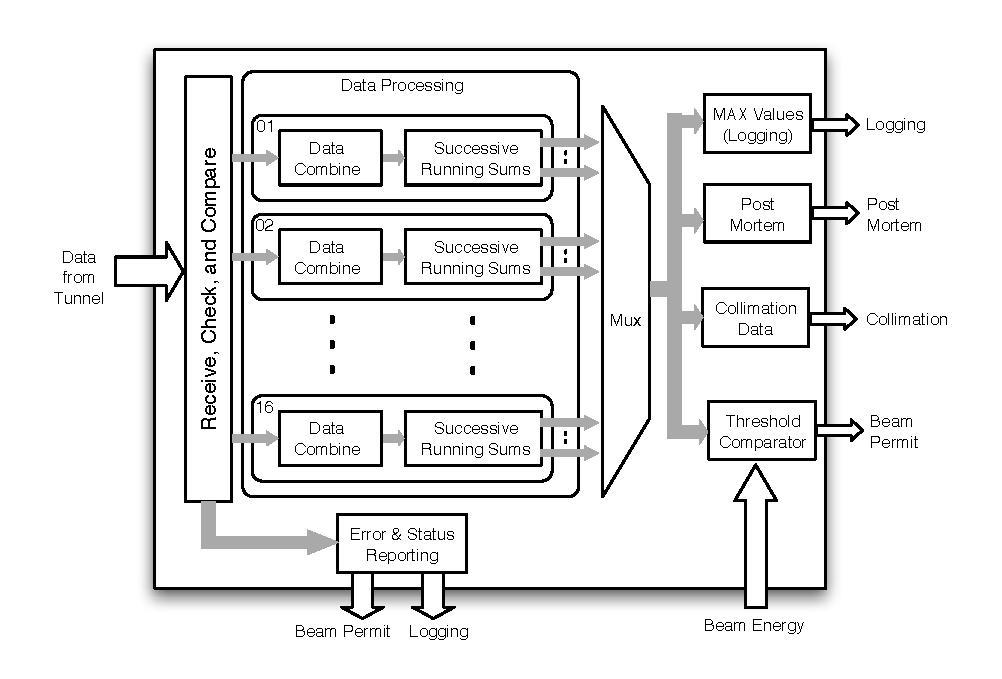
\includegraphics{BLETC.eps}}
   \caption{Block diagram of the processes assigned to BLETC card.}
  \label{fig:BLETC}
\end{figure}

The loss measurement principle \cite{Dehning-IPAC,Chris-FPGA} is based on the energy deposition detection of secondary shower particles using a specially-designed detector called \emph{ionization chamber}. There are around 4000 ionization chambers located under the magnets all around the tunnel. These detectors convert the signal given by the recording of shower particles into electrical signals and send them to tunnel cards. Tunnel cards, which are located in the tunnel and implemented by radiation-tolerant electronics, acquire and digitize the data from the detectors and transmit those to the surface using optical links. There, the data processing cards, named BLETCs, receive those data and decide whether or not the beam should be permitted to be injected or continue circulating. Each tunnel card receives data from eight detectors and each surface card receives data from two tunnel cards. The surface card provides data to the Logging, the Post Mortem and the Collimation systems that will be used to drive on-line displays in the control room to allow offline analysis of the losses and to setup automatically the collimators. Due to demanding performance requirements, the BLMS is implemented on modern FPGAs, which include the resources needed to design complex processing and can be reprogrammed making them ideal for future upgrades or system specification changes. Figure~\ref{fig:BLETC} shows a block diagram of the processes assigned in BLETC FPGA. In the following, we give a brief overview of each of the four main processing blocks in BLETC card.


\emph{(a) Receive, Check, and Compare (RCC)}: RCC is responsible for facilitating the reception process at the entry stage of the surface FPGA. It ensures the correct reception and detection of erroneous transmissions by redundancy in transmissions and using Cyclic Redundancy Check (CRC) and the 8B/10B algorithms.

\emph{(b) Data Processing}: Quench of magnets that result from proton loss depends on the loss duration and the beam energy. Given the tolerance acceptable for quench prevention, the quench threshold versus loss time is approximated with a minimum number of sliding integration windows (called \emph{Running Sums}) fulfilling the tolerance. In order to achieve the \emph{dynamic range} (i.e. the domain of variation of the beam losses) requested by the specification, the detectors use both Current-to-Frequency Converters (CFCs) and ADC circuitries. The data processing block merges these two types of data coming from the same detector into one value and send it to the SRS block. The implementation of the SRS is discussed in more detail in the next section.

\emph{(c) Threshold Comparator}: Every new calculated running sum need to be compared with the corresponding threshold that was chosen by the beam energy reading given that moment. The comparator will initiate a beam dump request if any of the running sums is higher than its corresponding threshold. The beam dump requests are forwarded to the Beam Interlock System which will initiate the beam dump. There are 12 running sums calculated for each 16 detector channels allocated to a BLETC card. The beam energy information is scaled into 32 levels (0.45 to 7 TeV) and each processing module will hold data only for those 16 detectors connected. That would give a total of 6,144 threshold values needed to be held on each card.

\emph{(d) Logging, Post Mortem and Collimation}:  To be able to trace back the loss signal development, BLM should store the loss measurement data. This data will be sent over the VME-bus for online viewing and storage by the Logging and Post-Mortem systems. For the purpose of supervision, the BLM system will drive an online event display to show error and status information recorded by tunnel electronics and the RCC process as well as the maximum loss rates seen by the running sums. BLETC card also provides data to Collimation system for the correct alignment and setup of the collimators.



\section{Successive Running Sums (SRS)}
\label{sec-SRS}

\begin{figure}[t]
  \centering 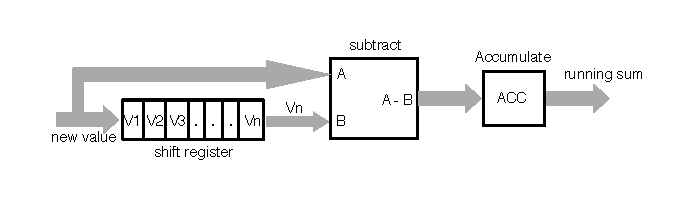
\includegraphics{rs.eps}
   \caption{Block diagram showing how to produce and maintain a continuous running sum of arriving values.}
  \label{fig:RS-basic}
\end{figure}

Beam losses can happen either in a single cycle of the beam in the tunnel, with a sudden beam loss, or in progressive losses during numerous cycles. One-cycle failures are called \emph{ultra-fast} losses. Multi-cycle losses can be divided between \emph{very fast} losses those which happen in less than 10 ms, \emph{fast} losses which happen in more than 10 ms and \emph{steady} losses, where the beam is lost over one second or more~\cite{Schmidt-ICFA}.


The processing of the data collected by the detectors involves a proper analysis of the loss patterns over time and a proper account of the energy of the beam. The procedure for the data processing is based on the idea that a constantly updated moving window can be kept by adding to a register the incoming newest value and subtracting its oldest value (see Figure~\ref{fig:RS-basic}). The number of values that are kept under the window defines the integration time it represents.  The ideal strategy is to have an infinite number of constantly updated moving windows with various lengths to cover the whole time region from 40 micro-seconds (the data arrival rate to BLETC card)  to 100 seconds for detecting ultra-fast losses to steady losses, respectively. Such an implementation is not feasible due to the limited amount of resources. Therefore, given the tolerance acceptable for quench prevention, the quench threshold versus loss time curve is approximated by a minimum number of steps that fulfill this tolerance.

\begin{figure}[t]
  \centering 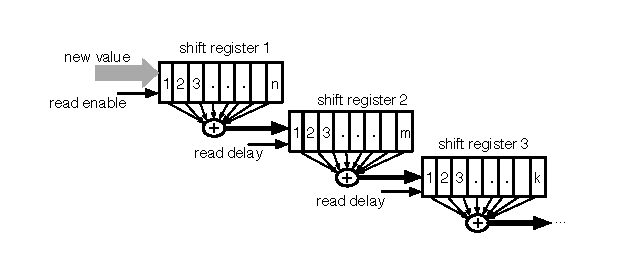
\includegraphics{SRS-basic.eps}
   \caption{Block diagram showing a configuration for efficient summation of many values.}
  \label{fig:SRS-basic}
\end{figure}


In order to construct long moving windows, it is required to keep long histories of received data, referred to as \emph{count} values. The technique employed to reach long integration periods with relatively small in length shift registers uses consecutive storage of sums of the counts. Instead of storing all values needed for the sum, this technique stores successively parts of the total sum using only a fraction of the otherwise needed memory space. This technique works by feeding the sum of one shift register's contents, every time its contents become completely updated, to the input of another shift register (see Figure~\ref{fig:SRS-basic}). By cascading more of these elements, very long moving windows could be constructed with significantly small memory space. The above scheme is the basis for the SRS implementation in BLETC.

SRS implementation minimizes the resource usage by using the already calculated running sums in order to calculate bigger in length running sums without the need of extra summation points. In addition, it makes use of multipoint shift registers that are configured to give intermediate outputs, referred to as \emph{taps}. The taps provide data outputs at certain points in the shift register chain thus contribute towards the efficient use of resources.

As in the SRS implementation the sum of one shift register's content is fed to the input of another shift register, the optimal achievable latency in the response of each stage is equal to the refreshing time of the preceding shift registers, i.e. the time needed to completely update its contents.  The \emph{read delay} signal (see Figure~\ref{fig:SRS-basic}) of each shift register holds a delay equal to this latency to guarantee the correct operation. Thus, the delay is every time equal to the preceding shift register's delay multiplied by the elements planned to be used in the sum.

\begin{figure}[t]
  \centering \scalebox{0.65}{ 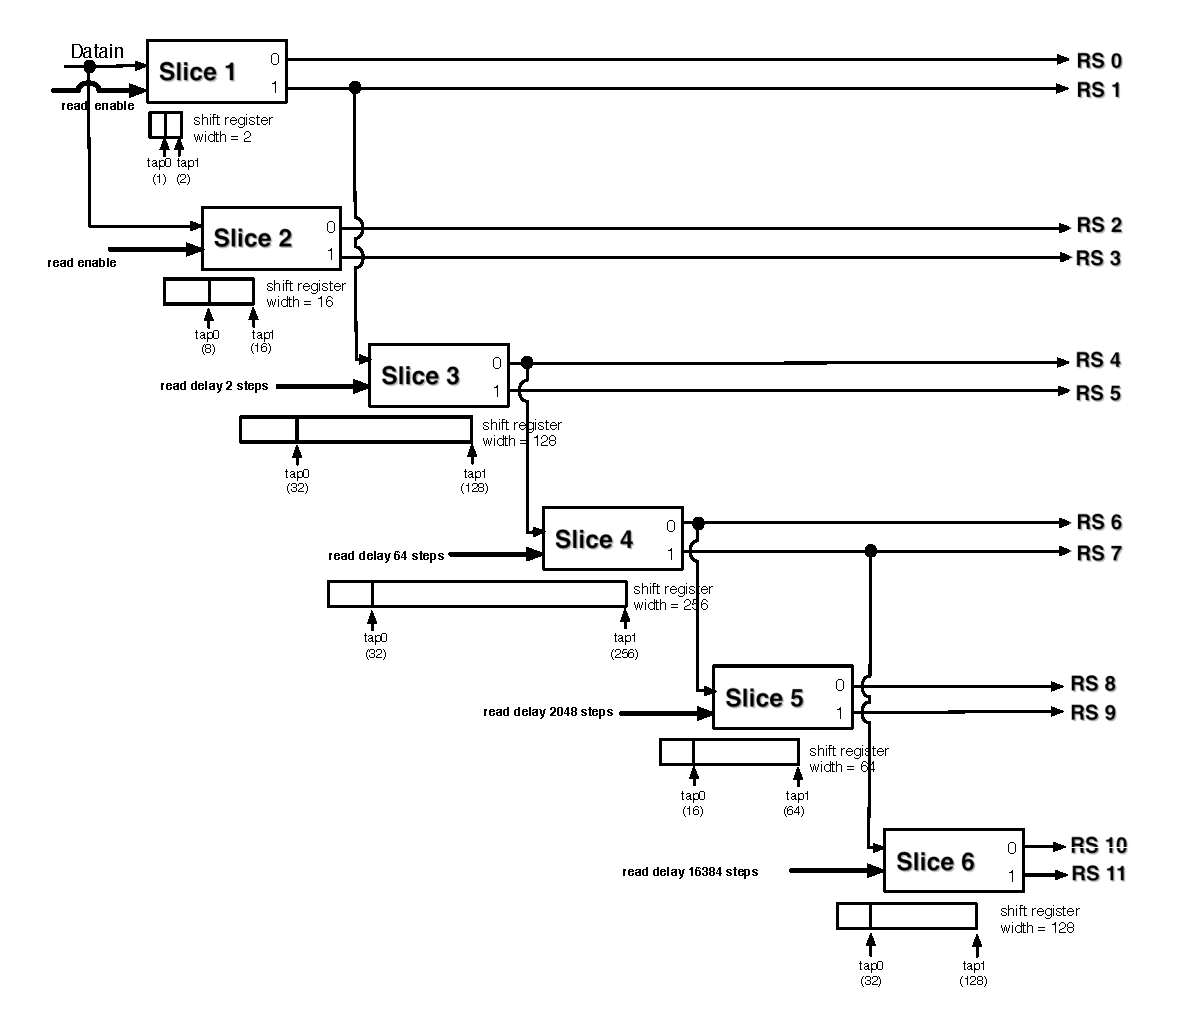
\includegraphics{srs-modified.eps}}
   \caption{The block diagram showing the Successive Running Sums implementation in BLETC card.}
  \label{fig:srs}
\end{figure}


Figure~\ref{fig:srs} shows the implementation of SRS in BLETC card. It consists of 6 \emph{slices}, where each slice computes two running sums (noted by RS) with the use of a multipoint shift register, two subtractors and two accumulators (see Figure~\ref{fig:slice}).

As shown in Table~\ref{}, by cascading 6 slices, it is enough to reach the 100 seconds upper integration limit requested by the specifications.

\begin{figure}[t]
  \centering \scalebox{0.8}{ 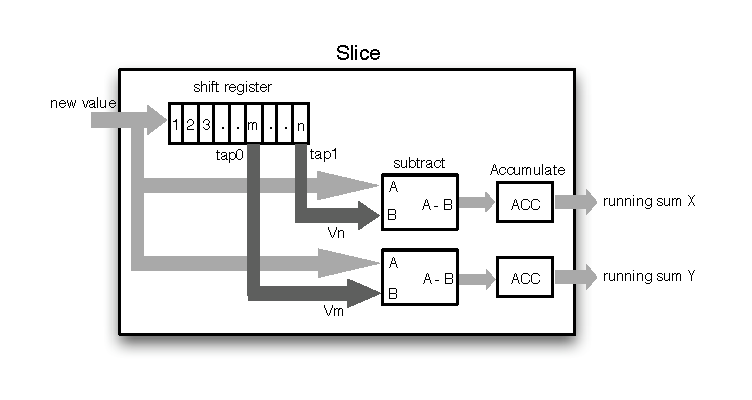
\includegraphics{multi-rs.eps}}
   \caption{The block diagram showing the implementation of each slice.}
  \label{fig:slice}
\end{figure}


\begin{figure}[t]
\centering
\begin{tabular}{|c|c|c|c|c|c|}
\hline
\multicolumn{2}{|c}{Range} &\multicolumn{2}{|c|}{Refreshing} & & \\\cline{1-4}
40 us steps & ms & 40 us steps  & ms & slice No & running sum \\\hline\hline
1 & 0.04 & 1 & 0.04 & & RS0 \\\hline
2 & 0.08 & 1 & 0.04 & & RS1 \\\hline
8 & 0.32 & 1 & 0.04 & slice 1 & RS2 \\\hline
16 & 0.64 & 1 & 0.04 & & RS3 \\\hline
64 & 2.56 & 2 & 0.08 & slice 2 & RS4 \\\hline
256 & 10.24 & 2 & 0.08 & & RS5 \\\hline
2048 & 81.92 & 64 & 2.56 &slice  3 & RS6 \\\hline
16384 & 655.36 & 64 & 2.56 &slice 3 & RS7 \\\hline
32768 &1310.72 & 2048 & 81.92 & slice 4 & RS8 \\\hline
131072 & 5242.88 & 2048 & 81.92 & slice 4 & RS9 \\\hline
524288 & 2097.52 & 16384 & 655.36 & slice 5 &RS10 \\\hline
2097152 & 83886.08 & 16384 & 655.36 & slice 5 & RS11 \\\hline

\end{tabular}
\vspace{0.04in}
\label{fig:example-bakery}
\caption{}
\end{figure}


\section{Verification of the SRS Implementation using HOL4}
\label{sec-verification}

%The calculation of running sums is a critical component of the BLMS.
%If there is no dangerous loss, the BLMS should not inhibit the beam.
%A false alarm costs at least three hours to resume operation, and compromises the availability of the system.
%However, if there is a dangerous loss, the BLMS must inhibit the beam.
%A quench due to dangerous loss costs at least 30 days of downtime.
%Thus, any error in the calculation compromises either the availability or the safety of the system.
%The current practice to check the correctness of the SRS is by simulation and testing.
%(isn't all this in the introduction now? is this the right place to repeat it/give more details?)
%In this paper we present a formal verification approach for the analysis of SRS implementation in BLM.

Our formal verification effort uses mechanised logical deduction, or \emph{theorem proving}.
In general, theorem proving is used to show that desired properties of a system are logically implied by a formal model of the system.
We use the HOL4 open source software tool~\cite{HOL4,DBLP:conf/tphol/SlindN08}, which was developed initially at the University of Cambridge, but now by an international team.
HOL4 enables the construction of theories in higher-order logic~\cite{DBLP:journals/jsyml/Church40}, a formal logic with a similar expressive power to set theory that is widely used for formalising hardware and software models and statements about them.
The implementation of HOL4 uses Milner's LCF approach~\cite{Milner:1972:LCF:891954}: a small ``kernel'' implementing the primitive rules of the logic, and convenient derived rules and tactics implemented in terms of the kernel.
Every theorem ultimately comes from the kernel, and this fact provides high assurance of the logical soundness of the verification results obtained using the system.

HOL4 is an \emph{interactive} theorem prover: the user provides the high level proof strategy by composing functions that automate common chains of logical deduction.
The work described here could have been done using other systems such as HOL Light~\cite{HOLLight,DBLP:conf/tphol/Harrison09a}, Isabelle/HOL~\cite{Isabelle}, ProofPower~\cite{ProofPower}, PVS~\cite{PVS,DBLP:conf/tphol/OwreS08} or Coq~\cite{Coq}.
The first three use essentially the same higher-order logic as HOL4, whilst PVS and Coq support more powerful logics.
%<What about ACL2?>
While offering less ``push-button'' automation than other kinds of formal verification such as model-checking, machine-assisted theorem proving is appropriate for verifying the SRS, since it is unlikely that the correctness theorems, which need lemmas proved by manually guided mathematical induction, could be generated automatically.

Our goal is to build a generic model of the SRS structure, and to prove that it satisfies its specification, that it calculates approximate running sums of received count values within acceptable error margins.
%Any statement in formal logic is necessarily precise, and one of our challenges has been characterizing our goal precisely.
%One of our challenges has been characterizing this goal precisely
Let $\mathsf{RS}\;n$ denote, as in Figure~\ref{fig:srs}, the output of slice $n$ in the SRS structure, which is supposed to compute a sum of received count values with some delay, and let $\mathsf{exact}\;n$ denote this sum.
A sketch of the desired correctness statement is \[\forall{n} \cdot \, \mathsf{RS}\;n= \mathsf{exact}\; n \pm\text{acceptable error}\]
Although Figure~\ref{fig:srs} suggests that the SRS structure has only twelve outputs  (i.e. $0\leq{n}\leq11$), we obtain a more generic result (that is useful in future upgrades of the system) by proving the correctness of the above statement for all values of $n$.

%To prove the equation above, we need to formalize all of its terms.
To make the above correctness statement more precise, we need to include the notion of time.
The count values arrive at the input of the SRS block every 40 micro-seconds, which we abstract as a single time step in our logical model.
We formalize the input stream as a function of time: $D\;t$ denotes the input value to the SRS structure at time $t$.
In addition, the terms in the above statement depend on this stream of input counts.
With these refinements, the correctness statement becomes: \[\forall{D\,n\,t} \cdot \,\mathsf{RS}\;D\;n\;t = \mathsf{exact}\;D\;\;n\;t\pm\text{acceptable error}\]

%First, we make two items explicit: that the equation is to be understood as holding at each time step, and that the terms depend on the stream of input counts over time.
%With these refinements, our statement becomes \[\forall{D\,n\,t}.\,\mathsf{RS}\;D\;n\;t=\text{sum, given input stream $D$, for output $n$ at time $t$}\pm\text{acceptable error}\]
%(The input stream is a function of time: $D\;t$ is the input value to the whole SRS structure at time $t$.)

%To formalize the term on the left hand side, we need to build a logical model of the SRS structure.
The first natural step to prove the correctness statement is to build a logical model of the SRS structure.
Our work proceeded in two phases, starting with a model of a simplified structure and proceeding to a model which is closer to the SRS implementation in BLMS.
In both phases, we model each building block of the SRS structure that holds a count value -- for example, each cell in each shift register -- as a function in HOL that takes the input stream and current time step as inputs and returns the value the corresponding building block holds at that time.

%In both cases, we represent each piece of the SRS structure that has a value---for example, each cell in each shift register---as a function in HOL that takes the global input stream and current time step as input and returns the value of the piece of the structure at that time.

Our simplifications in the first phase include:
\begin{enumerate}
\item Masking the middle taps in each slice,
\item Considering a more regular arrangement of slices than the SRS implementation in BLMS,
\item Masking the subtractors and the accumulators in each slice, instead, defining the output of a slice as the sum of the values in its cells directly,
\item Simplifying timing by ignoring some of the delays that each building block may introduce, {\bf this is not true - there were delays in the simplified model}
\item Using natural numbers, rather than finite words, for count values
\end{enumerate}

Building a logical model for simplified structure of the SRS helped us improve our understanding of the behavior of the SRS.
{\bf what else did we learn through this process? If there was no particular advantage, I don't think we should mention the simplified version.
(I don't think there was any particular advantage -- Ramana)}.

In the second phase, we eliminated the first four simplifications (listed above) by adding middle taps, a more flexible arrangement of slices, the subtractor and accumulator, and considering the delays that each block may introduce.
In both cases, however, the model is simultaneously a simplification and a generalization of the actual structure of SRS in BLMS in the following way: we model an infinite number of slices (rather than six slices), each with an infinite number of shift register cells and taps (rather than fixed width shift registers and only two taps), simply by letting indices range over the natural numbers without explicitly giving limits.
This parameterization makes the model and the analysis more likely to be applicable to future upgraded/modified versions of the system.

%%%%% upto here %%%
We describe the more realistic (second phase) model here.
Table~\ref{tab:descriptions} lists the names of the HOL functions we define and their intended meanings, and Figure~\ref{fig:definitions} gives their definitions.
For our correctness equation above, we only need the last entry in the table, $\mathsf{RS}$; the first two entries, $\mathsf{tap}$ and $\mathsf{input}$, enable us to specify the exact configuration of the structure, and the remaining entries are used as ``glue'' leading up to the definition of $\mathsf{RS}$.
By using these intermediary functions, every definition in Figure~\ref{fig:definitions} is \emph{local} (only talks about a small part of the overall SRS structure) and therefore is easy to verify against its intended meaning.

\begin{table}
\caption{
Descriptions of the HOL functions comprising our model of the SRS structure.
\label{tab:descriptions}
}
\begin{tabular}{lp{0.8\textwidth}}
Function&Intended meaning\\
\hline\\
\(\mathsf{tap}\;n\;x\)&The position of tap $x$ of slice $n$.\\
\(\mathsf{input}\;n\)&A pair $(n',x)$ indicating that the input to slice $n$ is output $x$ of slice $n'$.\\
\(\mathsf{delay}\;n\)&The number of time steps between updates of slice $n$.\\
\(\mathsf{update\_time}\;n\;t\)&A boolean indicating whether $t$ is an update time for slice $n$.\\
\(\mathsf{source}\;D\;n\;m\;t\)&The value of the cell that is the direct input to cell $m$ of slice $n$, at time $t$, given input stream $D$.\\
\(\mathsf{SR}\;D\;n\;m\;t\)&The value of cell $m$ of shift register $n$, at time $t$, given input stream $D$.\\
\(\mathsf{output}\;D\;n\;x\;t\)&The value of output $x$ of slice $n$, at time $t$, given input stream $D$.\\
\(\mathsf{RS}\;D\;n\;t\)&The value of Running Sum register $n$ at time $t$, given input stream $D$.
\end{tabular}
\end{table}

\begin{figure}
\caption{
Definitions of the HOL functions comprising our model of the SRS structure.
\(\mathsf{tap}\) and \(\mathsf{input}\) are defined to match Figure~\ref{fig:srs}, counting positions within a shift register from $0$.
Slice $0$ is a fake slice representing the global input; this enables a succinct definition of $\mathsf{source}$.
The definition of $\mathsf{input}$ when $n=0$ or when $n>6$ does not change the structure represented, so we use definitions convenient for proving theorems.
A similar comment applies to other definitions when $n$, representing a slice number, is $0$, or when $x$, representing a shift register position, is above $1$.
\label{fig:definitions}}
\begin{align*}
\mathsf{tap}\;0\;0&=0&\mathsf{tap}\;0\;x&=0\\
\mathsf{tap}\;1\;0&=1-1&\mathsf{tap}\;1\;x&=2-1\\
\mathsf{tap}\;2\;0&=8-1&\mathsf{tap}\;2\;x&=16-1\\
&\dots&\mathsf{tap}\;6\;x&=128-1\quad\text{(where $x>0$)}\\
\mathsf{input}\;0&=(0,0)&\mathsf{input}\;1&=(0,0)\\
\mathsf{input}\;2&=(0,0)&\mathsf{input}\;3&=(1,1)\\
\mathsf{input}\;4&=(3,0)&\mathsf{input}\;5&=(4,0)\\
\mathsf{input}\;6&=(4,1)&\mathsf{input}\;n&=(n-1,0)\quad\text{(where $n>6$)}
\end{align*}
\begin{align*}
\mathsf{delay}\;0&=1\\
\mathsf{delay}\;n&=\mathsf{delay}\;n'\times((\mathsf{tap}\;n'\;x)+1)\\
&\qquad\text{where $(n',x)=\mathsf{input\;n}$ (and $n>0$)}
\end{align*}
\begin{align*}
\mathsf{update\_time}\;n\;t&\iff(t\operatorname{mod}\mathsf{delay}\;n=0)
\end{align*}
\begin{align*}
\mathsf{source}\;D\;n\;0\;t&=\mathsf{output}\;D\;n'\;x\;t\quad\text{where $(n',x)=\mathsf{input\;n}$}\\
\mathsf{source}\;D\;n\;m\;t&=\;\mathsf{SR}\;D\;n\;(m-1)\;\quad\text{(where $m>0$)}
\end{align*}
\begin{align*}
\mathsf{output}\;D\;0\;x\;t&=D\;t\\
\mathsf{output}\;D\;n\;x\;0&=0\\
\mathsf{output}\;D\;n\;x\;t&=
\text{if $\mathsf{update\_time}\;n\;t$}\\
&\qquad\text{then }((\mathsf{output}\;D\;n\;x\;(t-1))+(\mathsf{source}\;D\;n\;0\;(t-1)))-(\mathsf{SR}\;D\;n(\mathsf{tap}\;n\;x)\;(t-1))\\
&\qquad\text{else }\mathsf{output}\;D\;n\;x\;(t-1)\qquad\text{(where $t>0$)}
\end{align*}
\begin{align*}
\mathsf{SR}\;D\;n\;m\;0&=0\\
\mathsf{SR}\;D\;n\;m\;t&=\text{if $\mathsf{update\_time}\;n\;t$}\\
&\qquad\text{then }\mathsf{source}\;D\;n\;m\;(t-1)\\
&\qquad\text{else }\mathsf{SR}\;D\;n\;m\;t\qquad\text{(where $t>0$)}
\end{align*}
\begin{align*}
\mathsf{RS}\;D\;n\;t&=\mathsf{output}\;D\;\left(\left\lfloor\frac{n}{2}\right\rfloor+1\right)\;(n\operatorname{mod}2)
\end{align*}
\end{figure}

%One of our objectives in formally modelling SRS was to keep the topology parameterized.
%It is likely that the configuration of the slices and shift registers will in the future change to accommodate higher precision.
%A parameterized model can be used both for current and future versions of the system.
%For this, we formalized the definitions of the model by six parameters:

\section{Conclusions and Lessons Learned}
\label{sec-conclusions}


\bibliographystyle{plain}
\bibliography{refs}


\end{document}

